% Options for packages loaded elsewhere
\PassOptionsToPackage{unicode}{hyperref}
\PassOptionsToPackage{hyphens}{url}
\PassOptionsToPackage{dvipsnames,svgnames,x11names}{xcolor}
%
\documentclass[fleqn,10pt]{wlscirep}

\usepackage{lineno}

\linenumbers


\usepackage{amsmath,amssymb}
\usepackage{iftex}
\ifPDFTeX
  \usepackage[T1]{fontenc}
  \usepackage[utf8]{inputenc}
  \usepackage{textcomp} % provide euro and other symbols
\else % if luatex or xetex
  \usepackage{unicode-math}
  \defaultfontfeatures{Scale=MatchLowercase}
  \defaultfontfeatures[\rmfamily]{Ligatures=TeX,Scale=1}
\fi
\usepackage{lmodern}
\ifPDFTeX\else  
    % xetex/luatex font selection
\fi
% Use upquote if available, for straight quotes in verbatim environments
\IfFileExists{upquote.sty}{\usepackage{upquote}}{}
\IfFileExists{microtype.sty}{% use microtype if available
  \usepackage[]{microtype}
  \UseMicrotypeSet[protrusion]{basicmath} % disable protrusion for tt fonts
}{}
\makeatletter
\@ifundefined{KOMAClassName}{% if non-KOMA class
  \IfFileExists{parskip.sty}{%
    \usepackage{parskip}
  }{% else
    \setlength{\parindent}{0pt}
    \setlength{\parskip}{6pt plus 2pt minus 1pt}}
}{% if KOMA class
  \KOMAoptions{parskip=half}}
\makeatother
\usepackage{xcolor}
\setlength{\emergencystretch}{3em} % prevent overfull lines
\setcounter{secnumdepth}{-\maxdimen} % remove section numbering
% Make \paragraph and \subparagraph free-standing
\ifx\paragraph\undefined\else
  \let\oldparagraph\paragraph
  \renewcommand{\paragraph}[1]{\oldparagraph{#1}\mbox{}}
\fi
\ifx\subparagraph\undefined\else
  \let\oldsubparagraph\subparagraph
  \renewcommand{\subparagraph}[1]{\oldsubparagraph{#1}\mbox{}}
\fi



\providecommand{\tightlist}{%
  \setlength{\itemsep}{0pt}\setlength{\parskip}{0pt}}
\usepackage{longtable,booktabs,array}
\usepackage{calc} % for calculating minipage widths
% Correct order of tables after \paragraph or \subparagraph
\usepackage{etoolbox}
\makeatletter
\patchcmd\longtable{\par}{\if@noskipsec\mbox{}\fi\par}{}{}
\makeatother
% Allow footnotes in longtable head/foot
\IfFileExists{footnotehyper.sty}{\usepackage{footnotehyper}}{\usepackage{footnote}}
\makesavenoteenv{longtable}

\usepackage{graphicx}
\makeatletter
\def\maxwidth{\ifdim\Gin@nat@width>\linewidth\linewidth\else\Gin@nat@width\fi}
\def\maxheight{\ifdim\Gin@nat@height>\textheight\textheight\else\Gin@nat@height\fi}
\makeatother
% Scale images if necessary, so that they will not overflow the page
% margins by default, and it is still possible to overwrite the defaults
% using explicit options in \includegraphics[width, height, ...]{}
\setkeys{Gin}{width=\maxwidth,height=\maxheight,keepaspectratio}
% Set default figure placement to htbp
\makeatletter
\def\fps@figure{htbp}
\makeatother



\usepackage{orcidlink}
\definecolor{mypink}{RGB}{219, 48, 122}
\RequirePackage[numbers,super]{natbib}
\makeatletter
\makeatother
\makeatletter
\makeatother
\makeatletter
\@ifpackageloaded{caption}{}{\usepackage{caption}}
\AtBeginDocument{%
\ifdefined\contentsname
  \renewcommand*\contentsname{Table of contents}
\else
  \newcommand\contentsname{Table of contents}
\fi
\ifdefined\listfigurename
  \renewcommand*\listfigurename{List of Figures}
\else
  \newcommand\listfigurename{List of Figures}
\fi
\ifdefined\listtablename
  \renewcommand*\listtablename{List of Tables}
\else
  \newcommand\listtablename{List of Tables}
\fi
\ifdefined\figurename
  \renewcommand*\figurename{Figure}
\else
  \newcommand\figurename{Figure}
\fi
\ifdefined\tablename
  \renewcommand*\tablename{Table}
\else
  \newcommand\tablename{Table}
\fi
}
\@ifpackageloaded{float}{}{\usepackage{float}}
\floatstyle{ruled}
\@ifundefined{c@chapter}{\newfloat{codelisting}{h}{lop}}{\newfloat{codelisting}{h}{lop}[chapter]}
\floatname{codelisting}{Listing}
\newcommand*\listoflistings{\listof{codelisting}{List of Listings}}
\makeatother
\makeatletter
\@ifpackageloaded{caption}{}{\usepackage{caption}}
\@ifpackageloaded{subcaption}{}{\usepackage{subcaption}}
\makeatother
\makeatletter
\@ifpackageloaded{tcolorbox}{}{\usepackage[skins,breakable]{tcolorbox}}
\makeatother
\makeatletter
\@ifundefined{shadecolor}{\definecolor{shadecolor}{rgb}{.97, .97, .97}}
\makeatother
\makeatletter
\makeatother
\makeatletter
\makeatother
\ifLuaTeX
  \usepackage{selnolig}  % disable illegal ligatures
\fi
\IfFileExists{bookmark.sty}{\usepackage{bookmark}}{\usepackage{hyperref}}
\IfFileExists{xurl.sty}{\usepackage{xurl}}{} % add URL line breaks if available
\urlstyle{same} % disable monospaced font for URLs
\hypersetup{
  pdftitle={Data Descriptor Title (110 character maximum, inc. spaces)},
  pdfauthor={Christine Author; Derek Author; Sam Author},
  pdfkeywords={keyword 1, keyword 2, keyword 3, keyword 4},
  colorlinks=true,
  linkcolor={blue},
  filecolor={Maroon},
  citecolor={Blue},
  urlcolor={blue},
  pdfcreator={LaTeX via pandoc}}


\title{Data Descriptor Title (110 character maximum, inc. spaces)}

                                                                                    \author[1\dag]{Christine
Author}
                                                                                                                                                \author[1\dag]{Derek
Author}
                                                                                                                                                \author[2*]{Sam
Author\orcidlink{0000-0001-1122-3555}}
                                                                
    \affil[1]{Big Old University, University Road, City, Country}
    \affil[2]{Research Institute, Main Road, City, Country}

                    \affil[*]{corresponding author(s): Sam Author Sam
Author@researchinst.org}
    
\affil[$\dag$]{these authors contributed equally to this work}

\begin{abstract}
This is a manuscript template for Data Descriptor submissions to
\textbf{Scientific Data} \url{http://www.nature.com/scientificdata}. The
abstract must be no longer than 170 words, and should succinctly
describe the study, the assay(s) performed, the resulting data, and the
reuse potential, but should not make any claims regarding new scientific
findings. No references are allowed in this section.
\end{abstract}
\begin{document}
\flushbottom
\maketitle
%  Click the title above to edit the author information and abstract

\thispagestyle{empty}\ifdefined\Shaded\renewenvironment{Shaded}{\begin{tcolorbox}[sharp corners, enhanced, boxrule=0pt, interior hidden, frame hidden, borderline west={3pt}{0pt}{shadecolor}, breakable]}{\end{tcolorbox}}\fi

Please note: Abbreviations should be introduced at the first mention in
the main text -- no abbreviations lists or tables should be included.
Structure of the main text is provided below.

\hypertarget{background-summary}{%
\section{Background \& Summary}\label{background-summary}}

(700 words maximum) An overview of the study design, the assay(s)
performed, and the created data, including any background information
needed to put this study in the context of previous work and the
literature. The section should also briefly outline the broader goals
that motivated the creation of this dataset and the potential reuse
value. We also encourage authors to include a figure that provides a
schematic overview of the study and assay(s) design. The Background \&
Summary should not include subheadings. This section and the other main
body sections of the manuscript should include citations to the
literature as needed.

\hypertarget{methods}{%
\section{Methods}\label{methods}}

The Methods should include detailed text describing any steps or
procedures used in producing the data, including full descriptions of
the experimental design, data acquisition assays, and any computational
processing (e.g.~normalization, image feature extraction). See the
detailed section in our submission guidelines for advice on writing a
transparent and reproducible methods section. Related methods should be
grouped under corresponding subheadings where possible, and methods
should be described in enough detail to allow other researchers to
interpret and repeat, if required, the full study. Specific data outputs
should be explicitly referenced via data citation (see Data Records and
Citing Data, below).

Authors should cite previous descriptions of the methods under use, but
ideally the method descriptions should be complete enough for others to
understand and reproduce the methods and processing steps without
referring to associated publications. There is no limit to the length of
the Methods section. Subheadings should not be numbered.

\hypertarget{subsection}{%
\subsection{Subsection}\label{subsection}}

Example text under a subsection. Bulleted lists may be used where
appropriate, e.g.

\begin{itemize}
\tightlist
\item
  First item
\item
  Second item
\end{itemize}

\hypertarget{third-level-subsection}{%
\subsubsection{Third-level subsection}\label{third-level-subsection}}

Topical subheadings are allowed.

\hypertarget{data-records}{%
\section{Data Records}\label{data-records}}

The Data Records section should be used to explain each data record
associated with this work, including the repository where this
information is stored, and to provide an overview of the data files and
their formats. Each external data record should be cited numerically in
the text of this section, for example \citep{Hao:gidmaps:2014}, and
included in the main reference list as described below. A data citation
should also be placed in the subsection of the Methods containing the
data-collection or analytical procedure(s) used to derive the
corresponding record. Providing a direct link to the dataset may also be
helpful to readers \url{https://doi.org/10.6084/m9.figshare.853801}.

Tables should be used to support the data records, and should clearly
indicate the samples and subjects (study inputs), their provenance, and
the experimental manipulations performed on each (please see `Tables'
below). They should also specify the data output resulting from each
data-collection or analytical step, should these form part of the
archived record.

\hypertarget{technical-validation}{%
\section{Technical Validation}\label{technical-validation}}

This section presents any experiments or analyses that are needed to
support the technical quality of the dataset. This section may be
supported by figures and tables, as needed. This is a required section;
authors must present information justifying the reliability of their
data.

\hypertarget{usage-notes}{%
\section{Usage Notes}\label{usage-notes}}

The Usage Notes should contain brief instructions to assist other
researchers with reuse of the data. This may include discussion of
software packages that are suitable for analysing the assay data files,
suggested downstream processing steps (e.g.~normalization, etc.), or
tips for integrating or comparing the data records with other datasets.
Authors are encouraged to provide code, programs or data-processing
workflows if they may help others understand or use the data. Please see
our code availability policy for advice on supplying custom code
alongside Data Descriptor manuscripts.

For studies involving privacy or safety controls on public access to the
data, this section should describe in detail these controls, including
how authors can apply to access the data, what criteria will be used to
determine who may access the data, and any limitations on data use.

\hypertarget{code-availability}{%
\section{Code availability}\label{code-availability}}

For all studies using custom code in the generation or processing of
datasets, a statement must be included under the heading ``Code
availability'', indicating whether and how the code can be accessed,
including any restrictions to access. This section should also include
information on the versions of any software used, if relevant, and any
specific variables or parameters used to generate, test, or process the
current dataset.

\hypertarget{references}{%
\section{References}\label{references}}

\renewcommand{\bibsection}{}
\bibliography{sample.bib}

\hypertarget{acknowledgements-not-compulsory}{%
\section{Acknowledgements (not
compulsory)}\label{acknowledgements-not-compulsory}}

Acknowledgements should be brief, and should not include thanks to
anonymous referees and editors, or effusive comments. Grant or
contribution numbers may be acknowledged.

\hypertarget{author-contributions-statement}{%
\section{Author contributions
statement}\label{author-contributions-statement}}

Must include all authors, identified by initials, for example: A.A.
conceived the experiment(s), A.A. and B.A. conducted the experiment(s),
C.A. and D.A. analysed the results. All authors reviewed the manuscript.

\hypertarget{competing-interests-mandatory-statement}{%
\section{Competing interests (mandatory
statement)}\label{competing-interests-mandatory-statement}}

The corresponding author is responsible for providing a
\href{https://www.nature.com/sdata/policies/editorial-and-publishing-policies\#competing}{competing
interest statement} on behalf of all authors of the paper. This
statement must be included in the submitted article file.

\hypertarget{figures-tables}{%
\section{Figures \& Tables}\label{figures-tables}}

Figures, tables, and their legends, should be included at the end of the
document. Figures and tables can be referenced in Quarto using
\texttt{!{[}caption{]}(source\_to\_figure.jpg)}, e.g.
Figure~\ref{fig-stream} and Table~\ref{tbl-example}.

\begin{figure}

{\centering 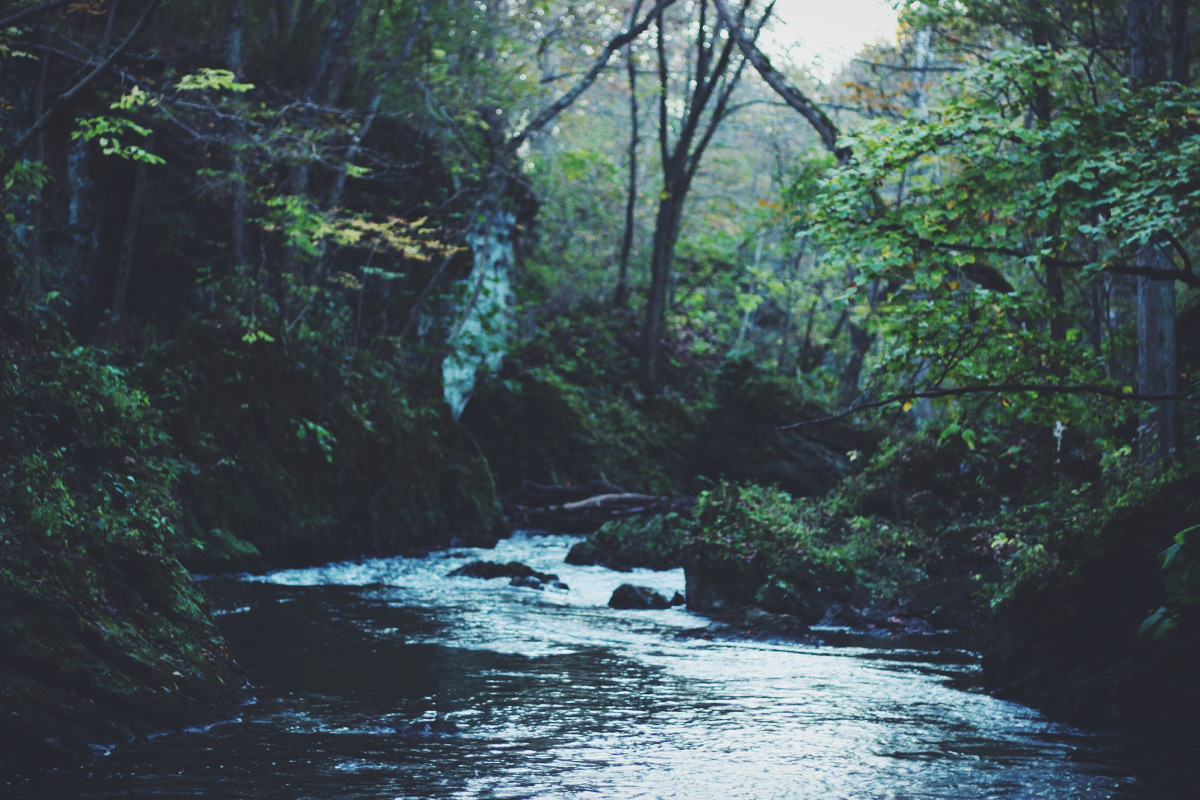
\includegraphics{stream.jpg}

}

\caption{\label{fig-stream}Legend (350 words max). Example legend text.}

\end{figure}

\hypertarget{tbl-example}{}
\begin{longtable}[]{@{}lll@{}}
\caption{\label{tbl-example}Legend (350 words max). Example legend
text.}\tabularnewline
\toprule\noalign{}
Condition & n & p \\
\midrule\noalign{}
\endfirsthead
\toprule\noalign{}
Condition & n & p \\
\midrule\noalign{}
\endhead
\bottomrule\noalign{}
\endlastfoot
A & 5 & 0.1 \\
B & 10 & 0.01 \\
\end{longtable}

Authors are encouraged to provide one or more tables that provide basic
information on the main `inputs' to the study (e.g.~samples,
participants, or information sources) and the main data outputs of the
study. Tables in the manuscript should generally not be used to present
primary data (i.e.~measurements). Tables containing primary data should
be submitted to an appropriate data repository.

Tables may be provided within the {\LaTeX} document or as separate files
(tab-delimited text or Excel files). Legends, where needed, should be
included here. Generally, a Data Descriptor should have fewer than ten
Tables, but more may be allowed when needed. Tables may be of any size,
but only Tables which fit onto a single printed page will be included in
the PDF version of the article (up to a maximum of three).

Due to typesetting constraints, tables that do not fit onto a single A4
page cannot be included in the PDF version of the article and will be
made available in the online version only. Any such tables must be
labelled in the text as `Online-only' tables and numbered separately
from the main table list e.g.~`Table 1, Table 2, Online-only Table 1'
etc.




\end{document}
